\subsection{Analysis}
\label{rpo:sec:analysis}

% \begin{table}[t]
    \caption{Narrowing down the Common Crawl to the candidate set used in our analysis (from left to right).}
    \label{rpo:tab:dataset_stats}
    \centering
    \footnotesize
    \begin{tabular}{lrrr}
    \toprule
    \multicolumn{2}{r}{\textbf{Relative CSS}} & \textbf{Alexa Top 1M} & \textbf{Candidate Set} \\
    \midrule
    All Pages & 203,609,675 & 141,384,967 & 136,793,450 \\
    Tested Pages & 53,725,270 & 31,448,446 & 30,991,702 \\
    Sites & 5,960,505 & 223,212 & 222,443 \\
    Document Types & 9,833 & 2,965 & 2,898 \\
    \bottomrule
    \end{tabular}
\end{table}


For the purposes of our analysis, we gradually narrow down the seed data from
the Common Crawl to pages using relative style paths in the Alexa Top 1\,M,
reflecting injected style directives under RPO, and being exploitable due to
quirks mode rendering.

% Table~\ref{rpo:tab:dataset_stats} shows a summary of our dataset. \textit{Tested
% Pages} refers to the set of randomly selected pages from the page groups as
% discussed in Section~\ref{rpo:sec:methodology:candidate}. For brevity,
% we are referring to \textit{Tested Pages} wherever we mention pages in the
% remainder of the paper.

\subsubsection{Relative Stylesheet Paths}
\label{rpo:sec:analysis:relative}

\begin{figure}[t]
\centering
\begin{minipage}{.32\textwidth}
    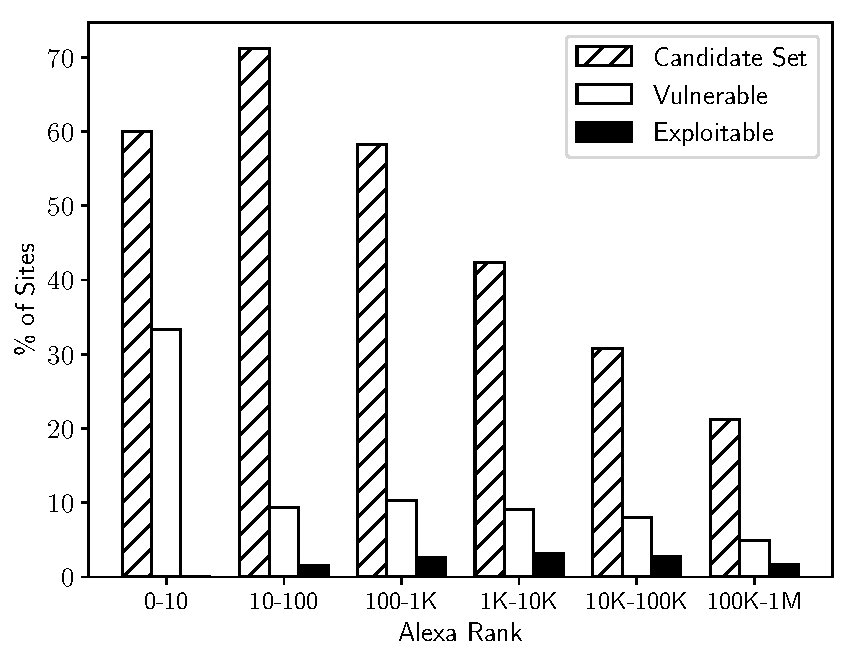
\includegraphics[width=1\textwidth,height=.8\textwidth]{rpo/figures/alexa_rank}
    \caption{Percentage of the Alexa site ranking in our candidate set
             (exponentially increasing bucket size).}
    \label{rpo:fig:analysis:alexa_rank}
\end{minipage}
\hfill
\begin{minipage}{.32\textwidth}
    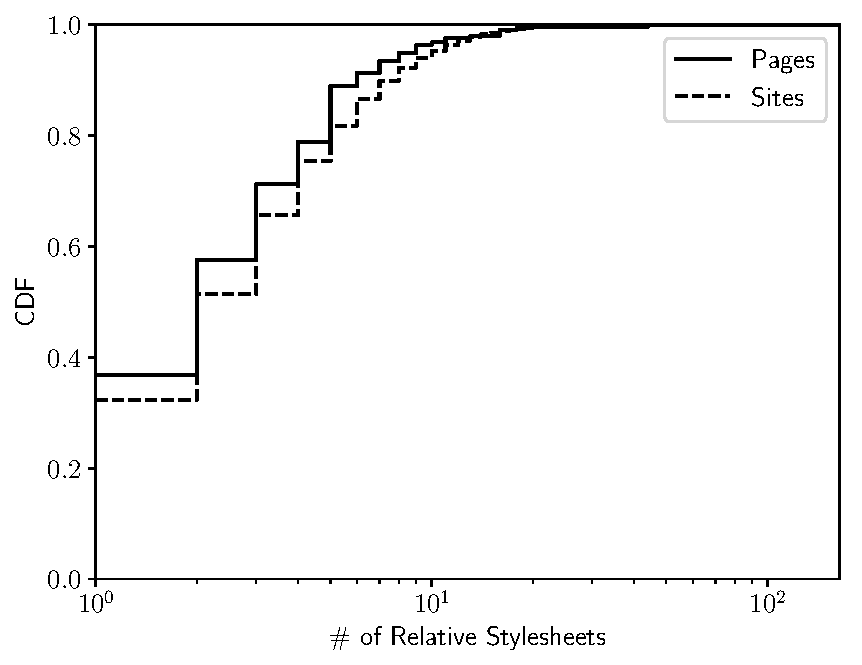
\includegraphics[width=1\textwidth,height=.8\textwidth]{rpo/figures/relative_stylesheets}
    \caption{CDF of total and maximum number of relative stylesheets per web
             page and site, respectively.}
    \label{rpo:fig:analysis:relative_stylesheets}
\end{minipage}
\hfill
\begin{minipage}{.32\textwidth}
    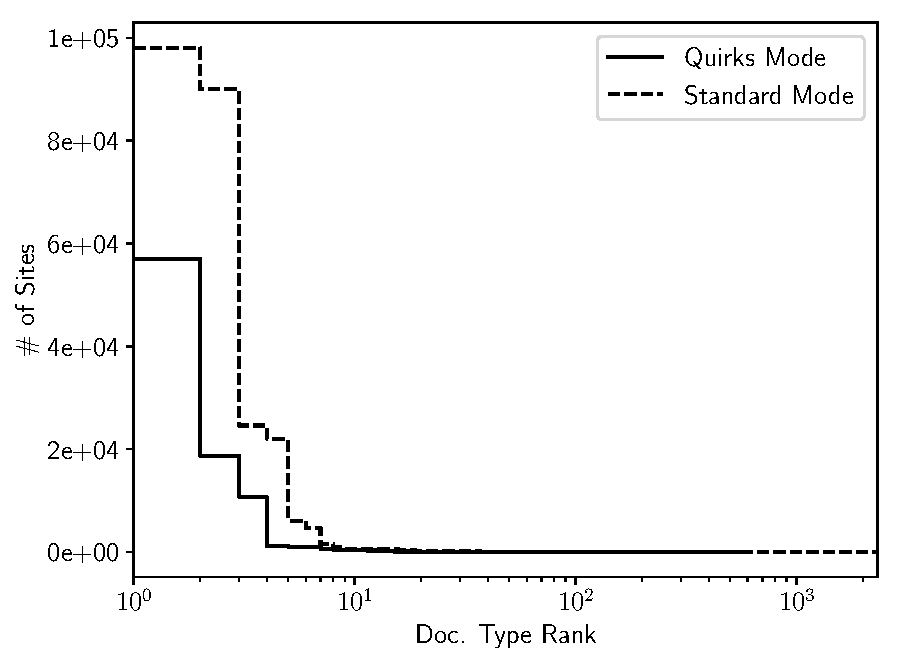
\includegraphics[width=1\textwidth,height=.8\textwidth]{rpo/figures/doctypes_rank_sites}
    \caption{Number of sites containing at least one page with a certain
             document type (ordered by doctype rank).}
    \label{rpo:fig:analysis:doctypes_rank_sites}
\end{minipage}
\end{figure}


To assess the extent to which our Common Crawl-seeded candidate set covers sites
of different popularity, consider the hatched bars in
Figure~\ref{rpo:fig:analysis:alexa_rank}. Six out of the ten largest sites
according to Alexa are represented in our candidate set. That is, they are
contained in the Common Crawl, and have relative style paths. The figure shows
that our candidate set contains a higher fraction of the largest sites and a
lower fraction of the smaller sites. Consequently, our results better represent
the most popular sites, which receive most visitors, and most potential victims
of RPO attacks.

While all the pages in the candidate set contain at least one relative
stylesheet path, Figure~\ref{rpo:fig:analysis:relative_stylesheets} shows that
63.1\,\% of them contain multiple relative paths, which increases the chances of
finding a successful RPO and style injection point.

\subsubsection{Vulnerable Pages}
\label{rpo:sec:analysis:vulnerable}

\begin{table*}[t]
    \centering
    \caption{Vulnerable/exploitable pages and sites in the candidate set (IE using framing).}
    \label{rpo:tab:vulnerable_exploitable_result}
    \footnotesize
    \begin{tabular}{lrrrrrr}
    \toprule
    \multirow{2}{*}{\textbf{Technique}} &
    \multicolumn{2}{c}{\textbf{Vulnerable}} &
    \multicolumn{2}{c}{\textbf{Exploitable (Chrome)}} &
    \multicolumn{2}{c}{\textbf{Exploitable (IE)}} \\

    \cmidrule[0.5pt](lr){2-3}
    \cmidrule[0.5pt](lr){4-5}
    \cmidrule[0.5pt](lr){6-7}

    &
    \textbf{Pages} &
    \textbf{Sites} &
    \textbf{Pages} &
    \textbf{Sites} &
    \textbf{Pages} &
    \textbf{Sites}
    \\

    \midrule

    Path Parameter & 309,079 (1.0\%) & 9,136 (4.1\%) & 6,048 (\textless 0.1\%) & 1,025 (0.5\%) & 52,344 (0.2\%) & 3,433 (1.5\%) \\
    Encoded Path & 53,502 (0.2\%) & 1,802 (0.8\%) & 3 (\textless 0.1\%) & 2 (\textless 0.1\%) & 24 (\textless 0.1\%) & 5 (\textless 0.1\%) \\
    Encoded Query & 89,757 (0.3\%) & 1,303 (0.6\%) & 23 (\textless 0.1\%) & 20 (\textless 0.1\%) & 137 (\textless 0.1\%) & 43 (\textless 0.1\%) \\
    Cookie & 15,656 (\textless 0.1\%) & 1,030 (0.5\%) & 4,722 (\textless 0.1\%) & 81 (\textless 0.1\%) & 2,447 (\textless 0.1\%) & 238 (0.1\%) \\

    \midrule

    Total & 377,043 (1.2\%) & 11,986 (5.4\%) & 10,781 (<0.1\%) & 1,106 (0.5\%) & 54,853 (0.2\%) & 3,645 (1.6\%) \\

    \bottomrule
    \end{tabular}

\end{table*}


We consider a candidate page vulnerable if one of the style injection techniques
of Section~\ref{rpo:sec:methodology:vulnerable} succeeds. In other
words, the server's response should reflect the injected payload. Furthermore,
we conservatively require that the response not contain a \texttt{base} tag
since a correctly configured base tag can prevent path confusion.

Table~\ref{rpo:tab:vulnerable_exploitable_result} shows that 1.2\,\% of pages
are vulnerable to at least one of the injection techniques, and 5.4\,\% of sites
contain at least one vulnerable page. The path parameter technique is most
effective against pages, followed by the encoded query and the encoded path
techniques. Sites that are ranked higher according to Alexa are more likely to
be vulnerable, as shown in Figure~\ref{rpo:fig:analysis:alexa_rank}, where
vulnerable and exploitable sites are relative to the candidate set in each
bucket. While one third of the candidate set in the Top~10 (two out of six
sites) is vulnerable, the percentage oscillates between 8 and 10\,\% among the
Top~100\,k. The candidate set is dominated by the smaller sites in the ranks
between 100\,k and 1\,M, which have a vulnerability rate of 4.9\,\% and push
down the average over the entire ranking.

% A \texttt{base} tag in the server response can prevent path confusion because it
% indicates how the browser should expand relative paths. We observed a number of
% inconsistencies with respect to its use. At first, 603 pages on 60 sites
% contained a \texttt{base} tag in their response; however, the server response
% after injecting our payload did not contain the tag anymore, rendering these
% pages potentially exploitable. Furthermore, Internet Explorer's implementation
% of the \texttt{base} tag appears to be broken. When such a tag is present,
% Internet Explorer fetches two URLs for stylesheets---one expanded according to
% the base URL specified in the tag, and one expanded in the regular, potentially
% ``confused'' way of using the page URL as the base. In our experiments, Internet
% Explorer always applied the ``confused'' stylesheet, even when the one based on
% the \texttt{base} tag URL loaded faster. Consequently, \texttt{base} tags do not
% appear to be an effective defense against RPO in Internet Explorer (They seem to
% work as expected in other browsers, including Edge).


\subsubsection{Exploitable Pages}
\label{rpo:sec:analysis:exploitable}

To test whether a vulnerable page was exploitable, we opened it in Chrome,
injected a style payload with an image reference (randomly generated URL), and
checked if the image was indeed loaded. This test succeeded for 2.9\,\% of
vulnerable pages; 0.5\,\% of sites in the candidate set had at least one
exploitable page (Table~\ref{rpo:tab:vulnerable_exploitable_result}).

% In the following, we explore various factors that may impact whether a
% vulnerable page can be exploited, and we show how some of these partial defenses
% can be bypassed.

% \paragraph{Document Types}
% \label{rpo:sec:analysis:doctypes}

% \begin{table}[t]
\centering
\begin{minipage}[t]{.55\textwidth}
    \caption{Summary of document type usage in sites.\newline}
    \label{rpo:tab:doctypes_summary}
    \centering
    \footnotesize
    \begin{tabular}{lrr}
    \toprule
    \textbf{Doc. Type} & \textbf{At Least One Page} & \textbf{All Pages} \\
    \midrule

    None & 56,985 (25.6\%) & 19,968 (9.0\%) \\
    Quirks & 27,794 (12.5\%) & 7,720 (3.5\%) \\
    None or Quirks & 71,597 (32.2\%) & 30,040 (13.5\%) \\
    \addlinespace
    Standards & 192,403 (86.5\%) & 150,846 (67.8\%) \\    
    \bottomrule
    \end{tabular}
\end{minipage}
\hfill
\begin{minipage}[t]{.43\textwidth}
    \caption{Quirks mode document types by browser.}
    \label{rpo:tab:doctypes_browsers}
    \centering
    \footnotesize
    \begin{tabular}{llr}
    \toprule

    \textbf{Browser} &
    \textbf{OS} &
    \textbf{Doc. Types} \\

    \midrule
    Chrome 55 & Linux & 1,378 (31.9\,\%) \\
    Opera 42 & Linux & 1,378 (31.9\,\%) \\
    Safari 10 & macOS & 1,378 (31.9\,\%) \\
    \addlinespace
    Firefox 50 & Linux & 1,326 (30.7\,\%) \\
    \addlinespace
    Edge 38 & Windows & 1,319 (30.5\,\%) \\
    IE 11 & Windows & 1,319 (30.5\,\%) \\
    \bottomrule
    \end{tabular}
\end{minipage}
\end{table}


% \begin{table}[t]
    \caption{Most frequent document types causing all browsers to render
    in quirks mode, as well as the sites that use at least one such
    document type.}
    \label{rpo:tab:top_quirksmode_doctypes}
    \centering
    \footnotesize
    \begin{tabular}{lrr}
    \toprule
    \textbf{Document Type (shortened)} & \textbf{Pages} & \textbf{Sites} \\
    \midrule
    (none) & 1,818,595 (5.9\,\%) & 56,985 (25.6\,\%) \\
    "-//W3C//DTD HTML 4.01 Transitional//EN" & 721,884 (2.3\,\%) & 18,648 (8.4\,\%) \\
    "-//W3C//DTD HTML 4.0 Transitional//EN" & 385,656 (1.2\,\%) & 11,566 (5.2\,\%) \\
    "-//W3C//DTD HTML 3.2 Final//EN" & 22,019 (<0.1\,\%) & 1,175 (0.5\,\%) \\
    "-//W3C//DTD HTML 3.2//EN" & 10,839 (<0.1\,\%) & 927 (0.4\,\%) \\
    \midrule
    All & 3,046,449 (9.6\,\%) & 71,597 (32.2\,\%) \\
    \bottomrule
    \end{tabular}
\end{table}


% HTML document types play a significant role in RPO-based style injection attacks
% because browsers typically parse resources with a non-CSS content type in a CSS
% context only when the page specifies an ancient or non-standard HTML document
% type (or none at all). The pages in our candidate set contain a total of 4,318
% distinct document types. However, the majority of these unique document types
% are not standardized and differ from the standardized ones only by small
% variations, such as forgotten spaces or misspellings.

% To determine how browsers interpret these document types (i.e., whether they
% cause them to render a page in standards or quirks mode), we designed a
% controlled experiment. For each unique document type, we set up a local page
% with a relative stylesheet path and carried out an RPO attack to inject CSS
% using a payload similar to what we described in
% Section~\ref{rpo:sec:methodology:vulnerable}. We automatically opened
% the local page in Chrome, Firefox, Edge, Internet Explorer, Safari, and Opera,
% and we kept track of which document type caused the injected CSS to be parsed
% and the injected background image to be downloaded.

% Table~\ref{rpo:tab:doctypes_browsers} contains the results of this experiment.
% Even though the exact numbers vary among browsers, roughly a third of the unique
% document types we encountered result in quirks mode rendering. Not surprisingly,
% both Microsoft products Edge and Internet Explorer exhibit identical results,
% whereas the common Webkit ancestry of Chrome, Opera, and Safari also show
% identical results. Overall, 1,271 (29.4\,\%) of the unique document types force
% all the browsers into quirks mode, whereas 1,378 (31.9\,\%) of them cause at
% least one browser to use quirks mode rendering.
% Table~\ref{rpo:tab:top_quirksmode_doctypes} shows the most frequently used
% document types that force all the browsers into quirks mode, which includes the
% absence of a document type declaration in the page.

% To test how often Internet Explorer allows a page's document type to be
% overridden when loading it in an \texttt{iframe}, we created another controlled
% experiment using a local attack page framing the victim page, as outlined in
% Section~\ref{rpo:sec:methodology:exploitable}. Using Internet
% Explorer~11, we loaded our local attack page for each unique document type
% inside the frame, and tested if the injected CSS was parsed. While Internet
% Explorer parsed the injected CSS for 1,319 (30.5\,\%) of the document types in
% the default setting, the frame override trick caused CSS parsing for 4,248
% (98.4\,\%) of the unique document types.

% While over one thousand document types result in quirks mode, and around three
% thousand document types cause standards mode parsing, the number of document
% types that have been standardized is several orders of magnitude smaller. In
% fact, only a few (standardized) document types are used frequently in pages,
% whereas the majority of unique document types are used very rarely.
% Figure~\ref{rpo:fig:analysis:doctypes_rank_sites} shows that only about ten
% standards and quirks mode document types are widely used in pages and sites.
% Furthermore, only about 9.6\,\% of pages in the candidate set use a quirks mode
% document type; on the remaining pages, potential RPO style injection
% vulnerabilities cannot be exploited because the CSS would not be parsed (unless
% Internet Explorer is used). However, when grouping pages in the candidate set by
% site, 32.2\,\% of sites contain at least one page rendered in quirks mode
% (Table~\ref{rpo:tab:doctypes_summary}), which is one of the preconditions for
% successful RPO.

% \paragraph{Internet Explorer Framing}

% We showed above that by loading a page in a frame, Internet Explorer can be
% forced to disregard a standards mode document type that would prevent
% interpretation of injected style. To find out how often this technique can be
% applied for successful RPO attacks, we replicated our Chrome experiment in
% Internet Explorer, this time loading each vulnerable page inside a frame. Around
% 14.5\,\% of vulnerable pages were exploitable in Internet Explorer, five times
% more than in Chrome (1.6\,\% of the sites in the candidate set).

% Figure~\ref{rpo:fig:analysis:alexa_rank} shows the combined exploitability
% results for Chrome and Internet Explorer according to the rank of the site.
% While our methodology did not find any exploitable vulnerability on the six
% highest-ranked sites in the candidate set, between 1.6\,\% and 3.2\,\% of
% candidate sites in each remaining bucket were found to be exploitable. The
% highest exploitability rate occurred in the ranks 1\,k through 10\,k.

% Broken down by injection technique, the framing trick in Internet Explorer
% results in more exploitable pages for each technique except for cookie injection
% (Table~\ref{rpo:tab:vulnerable_exploitable_result}). One possible explanation
% for this difference is that the Internet Explorer crawl was conducted one month
% after the Chrome crawl, and sites may have changed in the meantime. Furthermore,
% we observed two additional impediments to successful exploitation in Internet
% Explorer that do not apply to Chrome. The framing technique is susceptible to
% frame-busting methods employed by the framed pages, and Internet Explorer
% implements an anti-MIME-sniffing header that Chrome appears to ignore. We
% analyze these issues below.

% \paragraph{Anti-Framing Techniques}

% Some sites use a range of techniques to prevent other pages from loading them in
% a frame~\cite{w2sp2010frame_busting}. One of these techniques is the
% \texttt{X-Frame-Options} header. It accepts three different values:
% \texttt{DENY}, \texttt{SAMEORIGIN}, and \texttt{ALLOW-FROM} followed by a
% whitelist of URLs.

% In the vulnerable dataset, 4,999 pages across 391 sites use this header
% correctly and as a result prevent the attack. However, 1,900 pages across 34
% sites provide incorrect values for this header, and we successfully attack 552
% pages on 2 sites with Internet Explorer.

% A related technique is the \texttt{frame-ancestors} directive provided by
% Content Security Policy. It defines a (potentially empty) whitelist of URLs
% allowed to load the current page in a frame, similar to \texttt{ALLOW-FROM}.
% However, it is not supported by Internet Explorer, thus it cannot be used to
% prevent the attack.

% Furthermore, developers may use JavaScript code to prevent framing of a page.
% Yet, techniques exist to bypass this
% protection~\cite{owasp_clickjacking_defence}. In addition, the attacker can use
% the HTML 5 \texttt{sandbox} attribute in the \texttt{iframe} tag and omit the
% \texttt{allow-top-navigation} directive to render JavaScript frame-busting code
% ineffective. However, we did not implement any of these techniques to allow
% framing, which means that more vulnerable pages could likely be exploited in
% practice.

% \paragraph{MIME Sniffing}

% A consequence of self-reference in the type of RPO studied in this paper is that
% the HTTP content type of the fake ``stylesheet'' is \texttt{text/html} rather
% than the expected \texttt{text/css}. Because many sites contain misconfigured
% content types, many browsers attempt to infer the type based on the request
% context or file extension (\textit{MIME sniffing}), especially in quirks mode.
% In order to ask the browser to disable content sniffing and refuse interpreting
% data with an unexpected or wrong type, sites can set the header
% \texttt{X-Content-Type-Options: nosniff}~\cite{sp2009contentsniff,firefox_mime_sniff,content_type_options}.

% To determine whether the injected CSS is still being parsed and executed in
% presence of this header while the browser renders in quirks mode, we ran an
% experiment similar to Section~\ref{rpo:sec:analysis:doctypes}. For each browser
% in Table~\ref{rpo:tab:doctypes_browsers}, we extracted the document types in
% which the browser renders in quirks mode, and for each of them, we set up a
% local page with a relative stylesheet path. We then opened the page in the
% browser, launched an RPO attack, and monitored if the injected CSS was executed.

% Only Firefox, Internet Explorer, and Edge respected this header and did not
% interpret injected CSS in any of the quirks mode document types. The remaining
% browsers did not block the stylesheet even though the content type was not
% \texttt{text/css}. With an additional experiment, we confirmed that Internet
% Explorer blocked our injected CSS payload when \texttt{nosniff} was set, even in
% the case of the framing technique.

% Out of all the vulnerable pages, 96,618 pages across 232 sites had a
% \texttt{nosniff} response header; 23 pages across 10 sites were confirmed
% exploitable in Chrome but not in Internet Explorer, since the latter browser
% respects the header while the former does not.

% \subsubsection{Content Management Systems}
% \label{rpo:sec:analysis:cmses}

% While analyzing the exploitable pages in our dataset, we noticed that many
% appeared to belong to well-known CMSes. Since these web applications are
% typically installed on thousands of sites, fixing RPO weaknesses in these
% applications could have a large impact.

% To identify CMSes, we visited all exploitable pages using
% Wappalyzer~\cite{wappalyzer}. Additionally, we detected two CMSes that were not
% supported by Wappalyzer. Overall, we identified 23 CMSes on 41,288 pages across
% 1,589 sites. Afterwards, we manually investigated whether the RPO weakness
% stemmed from the CMS by installing the latest version of each CMS (or using the
% online demo), and testing whether exploitable paths found in our dataset were
% also exploitable in the CMS. After careful analysis, we confirmed four CMSes to
% be exploitable in their most recent version that are being used by 40,255 pages
% across 1,197 sites.

% Out of the four exploitable CMSes, one declares no document type and one uses a
% quirks mode document type. These two CMSes can be exploited in Chrome, whereas
% the remaining two can be exploited with the framing trick in Internet Explorer.
% % Beyond the view of our Common Crawl candidate set, Wappalyzer detected nearly
% % 32\,k installations of these CMSes across the Internet, which suggests that many
% % more sites could be attacked with RPO. We reported the RPO weaknesses to the
% % vendors of these CMSes using recommended notification
% % techniques~\cite{usenixsec2016vulnnotify1,usenixsec2016vulnnotify2,weis2017vulnnotify}.
% % Thus far, we heard back from one of the vendors, who acknowledged the
% % vulnerability and are going to take the necessary steps to fix the issue.
% % However, we have not received any response from the other vendors.

% \subsubsection{Mitigation Techniques}
% \label{rpo:sec:mitigation}

% Relative path overwrites rely on the web server and the web browser interpreting
% URLs differently. HTML pages can use only absolute (or root-relative) URLs,
% which removes the need for the web browser to expand relative paths.
% Alternatively, when the HTML page contains a \texttt{<base>} tag, browsers are
% expected to use the URL provided therein to expand relative paths instead of
% interpreting the current document's URL.
% % Both methods can remove ambiguities and
% % render RPO impossible if applied correctly. Specifically, base URLs must be set
% % according to the server's content routing logic. If developers choose to
% % calculate base URLs dynamically on the server side rather than setting them
% % manually to constant values, there is a risk that routing-agnostic algorithms
% % could be confused by manipulated URLs and re-introduce attack opportunities by
% % instructing browsers to use an attacker-controlled base URL. Furthermore,
% % Internet Explorer does not appear to implement this tag correctly.
% % 
% Web developers can reduce the attack surface of their sites by eliminating any
% injection sinks for strings that could be interpreted as a style directive.
% % However, doing so is challenging because in the attack presented in this paper,
% % style injection does not require a specific sink type and does not need the
% % ability of injecting markup. Injection can be accomplished with relatively
% % commonly used characters, that is, alphanumeric characters and
% % \texttt{()\{\}/"}. Experience has shown that despite years of efforts, even
% % context-sensitive and more special character-intensive XSS injection is still
% % possible in many sites, which leads us to believe that style injection will be
% % similarly difficult to eradicate. Even when all special characters in user input
% % are replaced by their corresponding HTML entities and direct style injection is
% % not possible, more targeted RPO attack variants referencing existing files may
% % still be feasible. For instance, it has been shown that user uploads of
% % seemingly benign profile pictures can be used as ``scripts'' (or
% % stylesheets)~\cite{rpo_techniques}.

% Instead of preventing RPO and style injection vulnerabilities, the most
% promising approach could be to avoid exploitation. In fact, declaring a modern
% document type that causes the HTML document to be rendered in standards mode
% makes the attack fail in all browsers except for Internet Explorer. Web
% developers can harden their pages against the frame-override technique in
% Internet Explorer by using commonly recommended HTTP headers.
% % \texttt{X-Content-Type-Options} to disable ``content type sniffing'' and always
% % use the MIME type sent by the server (which must be configured correctly),
% % \texttt{X-Frame-Options} to disallow loading the page in a frame, and
% % \texttt{X-UA-Compatible} to turn off Internet Explorer's compatibility view.
